\documentclass[00-main.tex]{subfiles}
% \standalonetrue
\setcounter{section}{4}
\pagestyle{footer}

\title{Alberi}

% arara: pdflatex: { draft: yes, synctex: no }
% arara: pdflatex: { synctex: yes }
% arara: latexmk: { clean: partial }
\begin{document}
% \maketitle

\section{Alberi}

% TODO scrivere introduzione

\subsubsection{Definizioni}

\begin{definition}[Albero radicato -- \foreign{rooted tree}]
Un albero consiste di un insieme di nodi e un insieme di archi orientati che connettono coppie di nodi, con le seguenti proprietà:
\begin{itemize}
	\item un nodo dell'albero è designato come nodo radice;
	\item ogni nodo \(n\), a parte la radice, ha esattamente un arco entrante;
	\item esiste un cammino unico dalla radice ad ogni nodo;
	\item l'albero è connesso.
\end{itemize}
\end{definition}

\begin{definition}[Albero radicato, definizione ricorsiva]
Un albero è dato da:
\begin{itemize}
	\item un insieme vuoto, oppure
	\item una radice e zero o più sottoalberi, ognuno dei quali è albero; la radice è connessa alla radice di ogni sottoalbero con un arco orientato.
\end{itemize}
\end{definition}

\begin{definition}[Profondità -- \foreign{depth}]
La lunghezza del cammino semplice dalla radice al nodo (misurato in archi).
\end{definition}

\begin{definition}[Livello -- \foreign{level}]
L'insieme dei nodi alla stessa profondità.
\end{definition}

\begin{definition}[Altezza dell'albero -- \foreign{height}]
La profondità massima delle sue foglie.
\end{definition}

\subsection{Terminologia}

\begin{minipage}[c]{.45\textwidth}
	\centering
	\begin{itemize}
		\item \(A\) è la radice (\foreign{root});
		\item \(B\), \(C\) sono radici dei sottoalberi (\foreign{roots of their subtrees});
		\item \(D\), \(E\) sono fratelli (\foreign{siblings});
		\item \(D\), \(E\) sono figli (\foreign{children}) di \(B\);
		\item \(B\) è il padre (\foreign{parent}) di \(D\), \(E\);
		\item \(H\), \(I\), \(J\), \(K\), \(L\), \(M\), \(G\) sono foglie (\foreign{leafs});
		\item gli altri nodi sono nodi interni (\foreign{internal nodes});
		\item \(E\) è lo zio di \(I\);
		\item \(B\) è il nonno di \(I\), \(I\) è il nipote di \(B\).
		% \item \(A\) è il bis-nonno di \(I\).
	\end{itemize}
\end{minipage}%
\begin{minipage}[c]{.45\textwidth}
	\centering
	\scalebox{.9}{
		\begin{forest} circled, wide
			[A [B [D [H][I]] [E [J][K]] ] [C [F [L][M]] [G] ]]
		\end{forest}
	}
\end{minipage}

\subsection{Alberi binari}

\begin{definition}[Albero binario]
Un albero binario è un albero radicato in cui ogni nodo ha al massimo due figli, che vengono identificati come figlio sinistro e figlio destro.
\end{definition}

\begin{note}
Due alberi \(T\) e \(U\) che hanno gli stessi nodi, gli stessi figli per ogni nodo e la stessa radice, sono distinti qualora un nodo \(u\) sia designato come figlio sinistro di un nodo \(v\) in \(T\) come figlio destro del medesimo nodo in \(U\).
In altre parole, anche se due alberi hanno lo stesso numero di nodi ed ognuno di questi nodi ha lo stesso numero di figli non è che detto che l'albero risultante sia identico.
\end{note}

\includestandalone{assets/algorithms/05/tree-binary-interface}

\subsubsection{Memorizzazione di un albero binario}

\begin{figure}[H]
	\centering
	\input{assets/figures/05/binary-tree}
\end{figure}

Vengono memorizzati i seguenti campi:
\begin{itemize}
	\item \emph{parent}: riferimento al nodo padre;
	\item \emph{left}: riferimento al figlio sinistro;
	\item \emph{right}: riferimento al figlio destro.
\end{itemize}
Uno qualunque di questi oggetti potrebbe essere pari a \Nil, stando ad indicare che sotto di sé non esiste nessun sottoalbero.

\subsubsection{Implementazione}

\includestandalone{assets/algorithms/05/tree-pseudocode}

\subsubsection{Visite}

La visita di un albero (o la ricerca) è una strategia per passare attraverso (visitare) tutti i nodi di un albero.
Si possono distinguere due tipi di visite:
\begin{enumerate}
	\item visita in profondità: chiamata anche \foreign{Deep-First Search} (DFS), per visitare un albero visita ricorsivamente ognuno dei suoi sottoalberi; esistono tre varianti in base a quando il nodo viene visitato (in pre, in o post order); questa particolare visita richiede il meccanismo di una pila (\foreign{stack});
	\item visita in ampiezza: chiamata anche \foreign{Breadth First Search} (BFS), per visitare un albero visita ogni livello, uno dopo l'altro partendo dalla radice; richiede il meccanismo di una coda (\foreign{queue}).
\end{enumerate}

A seconda di dove scrivo il codice in questo schema ottengo una visita diversa.

\includestandalone{assets/algorithms/05/dfsSchema}

\subsubsection{Applicazioni}

In genere post-visita e in-visita sono quelle più applicate, la pre-visita meno.

\subsubsection*{Visita in post-ordine}

Una possibile applicazione della visita post-ordine è quella di effettuare un conteggio dei nodi presenti nell'albero.

\includestandalone{assets/algorithms/05/conteggioNodi}

\subsubsection*{Visita in ordine (in-visita)}

\includestandalone{assets/algorithms/05/stampaEspressioni}

\subsubsection*{Complessità di una visita}

Il costo di una visita di un albero contenente \(n\) nodi è \(\Theta(n)\), in quanto ogni nodo viene visitato al massimo una volta.

\subsection{Alberi generici}

\includestandalone{assets/algorithms/05/tree-generic-interface}

\subsubsection{Visita in profondità}

Un albero binario è anche un albero generale e lo visitiamo esattamente come lo visitavamo prima.

\includestandalone{assets/algorithms/05/dfs}

\subsubsection{Visita in ampiezza}

Mentre nella visita in profondità la pila (\foreign{stack}) era implicita nella chiamata ricorsiva, in questo caso è necessario utilizzare \emph{esplicitamente} una coda (\foreign{queue}).
Un'altra differenza fra i due algoritmi è che l'algoritmo di visita in profondità era un algoritmo ricorsivo, mentre questo è iterativo.

\includestandalone{assets/algorithms/05/bfs}

\paragraph{Commento}
Mettiamo in coda tutti i nodi che vogliamo visitare passo passo.
Qui la stampa è in pre-visita ma qui -- a differenza dei grafi -- non ha molta importanza se la visita la facciamo prima o dopo.
Visito tutti i figli prima di passare al livello successivo.

\subsection{Memorizzazione}

Esistono diversi modi per memorizzare un albero, più o meno indicati a seconda del numero massimo e medio di figli presenti.
Le realizzazioni possibili sono:
\begin{enumerate}
	\item con vettore dei figli;
	\item primo figlio, prossimo fratello;
	\item con vettore dei padri
\end{enumerate}

\subsubsection{Realizzazione con vettore dei figli}

\begin{figure}[H]
	\centering
	\includegraphics[width=\textwidth]{assets/figures/05/tree-vectorChildren}
	\caption{Realizzazione con vettore dei figli}
	\label{fig:tree-vector-children}
\end{figure}

Vengono memorizzati i seguenti campi:
\begin{itemize}
	\item \emph{parent} che è il riferimento al nodo padre;
	\item vettore dei figli il quale a seconda del numero dei figli può comportare una discreta quantità di spazio sprecato.
\end{itemize}

\subsubsection{Realizzazione basata su Primo figlio, prossimo fratello}

Viene implementato come una lista di fratelli.

\begin{figure}[H]
	\centering
	\includegraphics[width=.8\textwidth]{assets/figures/05/tree-listChildren}
	\caption{Realizzazione basata su Primo figlio, prossimo fratello}
	\label{fig:tree-list-children}
\end{figure}

La memorizzazione che viene utilizzata nel file system è esattamente quella che ci siamo dati.

\includestandalone{assets/algorithms/05/tree-listChildren-interface}

\subsubsection{Realizzazione con vettore dei padri}

Nella Realizzazione con vettore dei padri l'albero è rappresentato da un vettore i cui elementi contengono il valore associato al nodo e l'indice della posizione del padre del vettore.

\bigskip
\begin{minipage}[c]{.5\textwidth}
	\centering
	\documentclass[tikz, varwidth=6in]{standalone}

% arara: pdflatex: { interaction: batchmode }
% arara: latexmk: { clean: partial }
\begin{document}

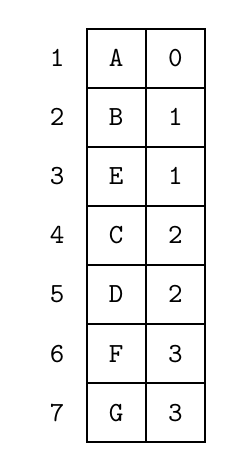
\begin{tikzpicture}[
	thick,
	font=\ttfamily\bfseries,
	minimum/.style={
		minimum width = 0.75cm,
		minimum height = 0.75cm
	},
	box/.style={
		draw,
		rectangle,
		inner sep =+ 0pt,
		minimum
	}
]
\node[box] at (0.00,-0.00) {A};
\node[box] at (0.75,-0.00) {0};
\node[box] at (0.00,-0.75) {B};
\node[box] at (0.75,-0.75) {1};
\node[box] at (0.00,-1.50) {E};
\node[box] at (0.75,-1.50) {1};
\node[box] at (0.00,-2.25) {C};
\node[box] at (0.75,-2.25) {2};
\node[box] at (0.00,-3.00) {D};
\node[box] at (0.75,-3.00) {2};
\node[box] at (0.00,-3.75) {F};
\node[box] at (0.75,-3.75) {3};
\node[box] at (0.00,-4.50) {G};
\node[box] at (0.75,-4.50) {3};

\node[minimum] at (-0.75,-0.00) {1};
\node[minimum] at (-0.75,-0.75) {2};
\node[minimum] at (-0.75,-1.50) {3};
\node[minimum] at (-0.75,-2.25) {4};
\node[minimum] at (-0.75,-3.00) {5};
\node[minimum] at (-0.75,-3.75) {6};
\node[minimum] at (-0.75,-4.50) {7};

\end{tikzpicture}
\end{document}

\end{minipage}%
\begin{minipage}[c]{.5\textwidth}
	\centering
	\begin{forest} circled, wide
	[\textsc{a}[\textsc{b}[\textsc{c}][\textsc{d}]][\textsc{e}[\textsc{f}][\textsc{g}]]]
	\end{forest}
\end{minipage}

\bigskip
Questa realizzazione può sembrare particolarmente assurda poiché dato un nodo non permette di stabilire direttamente quali sono i suoi figli, ma ci sono molti algoritmi che sono interessati solo ai padri.
Questa la rappresentazione più compatta che possiamo creare, vedremo la sua utilità quando andremo a studiare le visite sui grafi.
\end{document}
